

\hypertarget{the-complexity-of-the-morphogenesis}{%
\section{The complexity of the
morphogenesis}\label{the-complexity-of-the-morphogenesis}}

Epithelial cells play a crucial role in the formation of transient structures during embryonic development, such as the neural tube, somites, and precardiac epithelium, which serve as the precursor for the development of complex organs. During this process, different types of epithelia acquire distinct morphological forms and perform specific functions, including branched lungs, looped gut, kidney tubules, thyroid follicles, and sinusoids in the liver. The regulation of epithelial morphogenesis is a complex and hierarchical process that involves coordinated events at multiple spatial and temporal scales \cite{trepat2018}.

Some processes appear to be happening fast at the local level, such as cell shape changes through apical constrictions, which lead to global changes, such as the formation of a ventral furrow in a Drosophila embryo \cite{martin2009}. At the same time, chemical signaling events that activate these processes are slow and occur at a global level. The same complexity can be seen in\textit{ in vitro} systems, where a cluster of dissociated stem cells can assemble into an organoid or gastruloid and undergo global folds in response to appropriate culture conditions \cite{collinet2021}.

The underlying mechanisms of epithelial morphogenesis are intricate and involve multiple factors, including genes responding to morphogen gradients, molecular machinery involved in apical constriction, and mechanical stresses that cause tissue-scale deformations. To fully understand the phenomenon of epithelial morphogenesis, it is essential to study these processes in detail, at multiple levels of complexity \cite{schock2002, lecuit2011}.

Rudolf Virchow's third tenet of the cell theory states that ``omnis cellula e cellula,'' meaning ``all cells come from cells'' \cite{virchow1860}.
\footnote{The famous epigram was coined by François-Vincent Raspail. Virchow is regarded as influential biomedical scientist of 19th century, but more interesting part is as a radical who took part in the March revolution of 1848. He was one of the first to advocate for the social origins of illness \cite{wright2012, brown2006}.}
Although all tissues originate from cells that contain essentially the same genetic information, each tissue has a distinct architecture and function. This raises several questions, such as: what makes cells different from each other? Are differences due to genes, environmental factors, or both? What drives shape changes in tissue morphogenesis? Over the last two centuries, the field of developmental biology has addressed many of these questions, but it has also raised new issues and left others unanswered.

Until last decade, the focus of the field had been on tracking and mapping patterns of cell movements to patterns of gene or protein expression \cite{gorfinkiel2021}. While these studies are influential and important for understanding morphogenetic patterns, they fall short in explaining how cells and tissues are physically shaped \cite{veenvliet2021, odell1981}. This is because the physical understanding of tissues has been limited to kinematic descriptions, which only describe tissue deformation or cell motion. However, we know that cells and tissues actively drive shape changes and movements through the generation of mechanical forces \cite{lecuit2011}. Thus, to have an integrated understanding of morphogenesis, we must consider the role of forces and mechanics.

\hypertarget{on-growth-and-form}{%
\section{On growth and form}\label{on-growth-and-form}}

Throughout history, the form of both animate and inanimate objects has been closely linked to their intended function. In fact, the 20th-century architectural principle `form follows function' highlights the idea that the organization of a structure should be based on its intended purpose. However, in developmental biology, the relationship between form and function is more complicated. For instance, self-assembling systems such as intestinal organoids, cancer spheroids, and gastruloids are perfect examples of this relationship, as each structure emerges from a set of cells in a suitable environment, adapting to perform a specific biological function \cite{gjorevski2016, ishiguro2017, morizane2017, vianello2019}. However, in numerous \textit{in vitro} experiments that involve a controlled cellular environment, the opposite principle appears to be at work. In these experiments, geometric constraints appear to drive biological function \cite{xi2018}. For example, seeding stem cells in a bio-printed three-dimensional geometry of the gastrointestinal tract can lead to the production of functional tissues with physiological characteristics of the intestine. The curvature of the structure can even control the formation of villus-like structures \cite{brassard2021}. 

\begin{figure}[h!]
	\centering
	\includegraphics[width=\textwidth]{chap2shah.png}
	\caption{\label{fig_2_1} \textbf{Multiscale imaging and tracking of embryo cell dynamics}: Top panels show in toto imaging of germlayer specification; red is mesendoderm, blue is epiblast, and yellow is endoderm. Bottom panel shows data analysis of long term pan embryo cell dynamics \cite{shah2019}}
\end{figure}

In a way, assembly of biological systems treads the line between self-organization and programmed material. Advanced microscopy techniques have allowed us to witness the intricacies of developmental processes with unprecedented clarity (see fig \ref{fig_2_1}). We can now observe cells and their motion throughout the morphogenetic process, from the formation of a spherical embryo to the creation of a complete organism \cite{shah2019}. Cells undergo shape changes and large-scale flows as they undergo morphogenesis, driven by mechanical forces in concert with biochemical processes \cite{labernadie2018, trepat2018, lecuit2011}. Thus, the dichotomy of form and function is incomplete without considering the physical laws of mechanics.


Over a century ago, D'Arcy Wentworth Thompson wrote the influential book ``On Growth and Form'' \cite{thompson1979}, in which he explored the relationship between geometry, physics, and biology in the context of morphogenesis. Thompson used examples to show how mathematical principles can explain biological phenomena, such as his theory of transformations, which demonstrates how related species can be represented geometrically (see fig \ref{fig_2_1b}). According to Thompson's daughter, he even used to draw pictures of dogs on rubber sheets and stretch them to show children how poodles could become dachshunds \cite{wolfram2022}. This distortion of shape represents significant alterations in various forces or rates of growth throughout the developmental processes of different organisms.

Thompson's approach was highly speculative, but his goal was to identify general principles behind the diverse forms and patterns found in biology. He compared growth curves of haddock, trees, and tadpoles, and found logarithmic spirals in shells, horns, and leaf arrangements.
\footnote{Funnily, He criticized the zoologists and morphologists of the time of assigning shapes to psychical instinct of the organism or some divine interference for creating the perfect shapes: “He finds a simple geometric construction, for instance in the honeycomb structure, he would fain refer it to psychical instinct or design rather than in the operation of physical forces. ... When he sees in snail, or nautilus, or tiny foraminiferal or radiolarian shell a close approach to sphere or spiral, he is prone of old habit to believe that after all it is something more than a spiral or a sphere, and that in this "something more" there lies what neither mathematics nor physics can explain}
Essentially, this book emphasized two points: first, all material forms of living things---cells, tissues, and organs---must obey the laws of physics, and second, quantitative measurements are necessary to unravel the physical principles of biology.

\begin{figure}[h!]
	\centering
	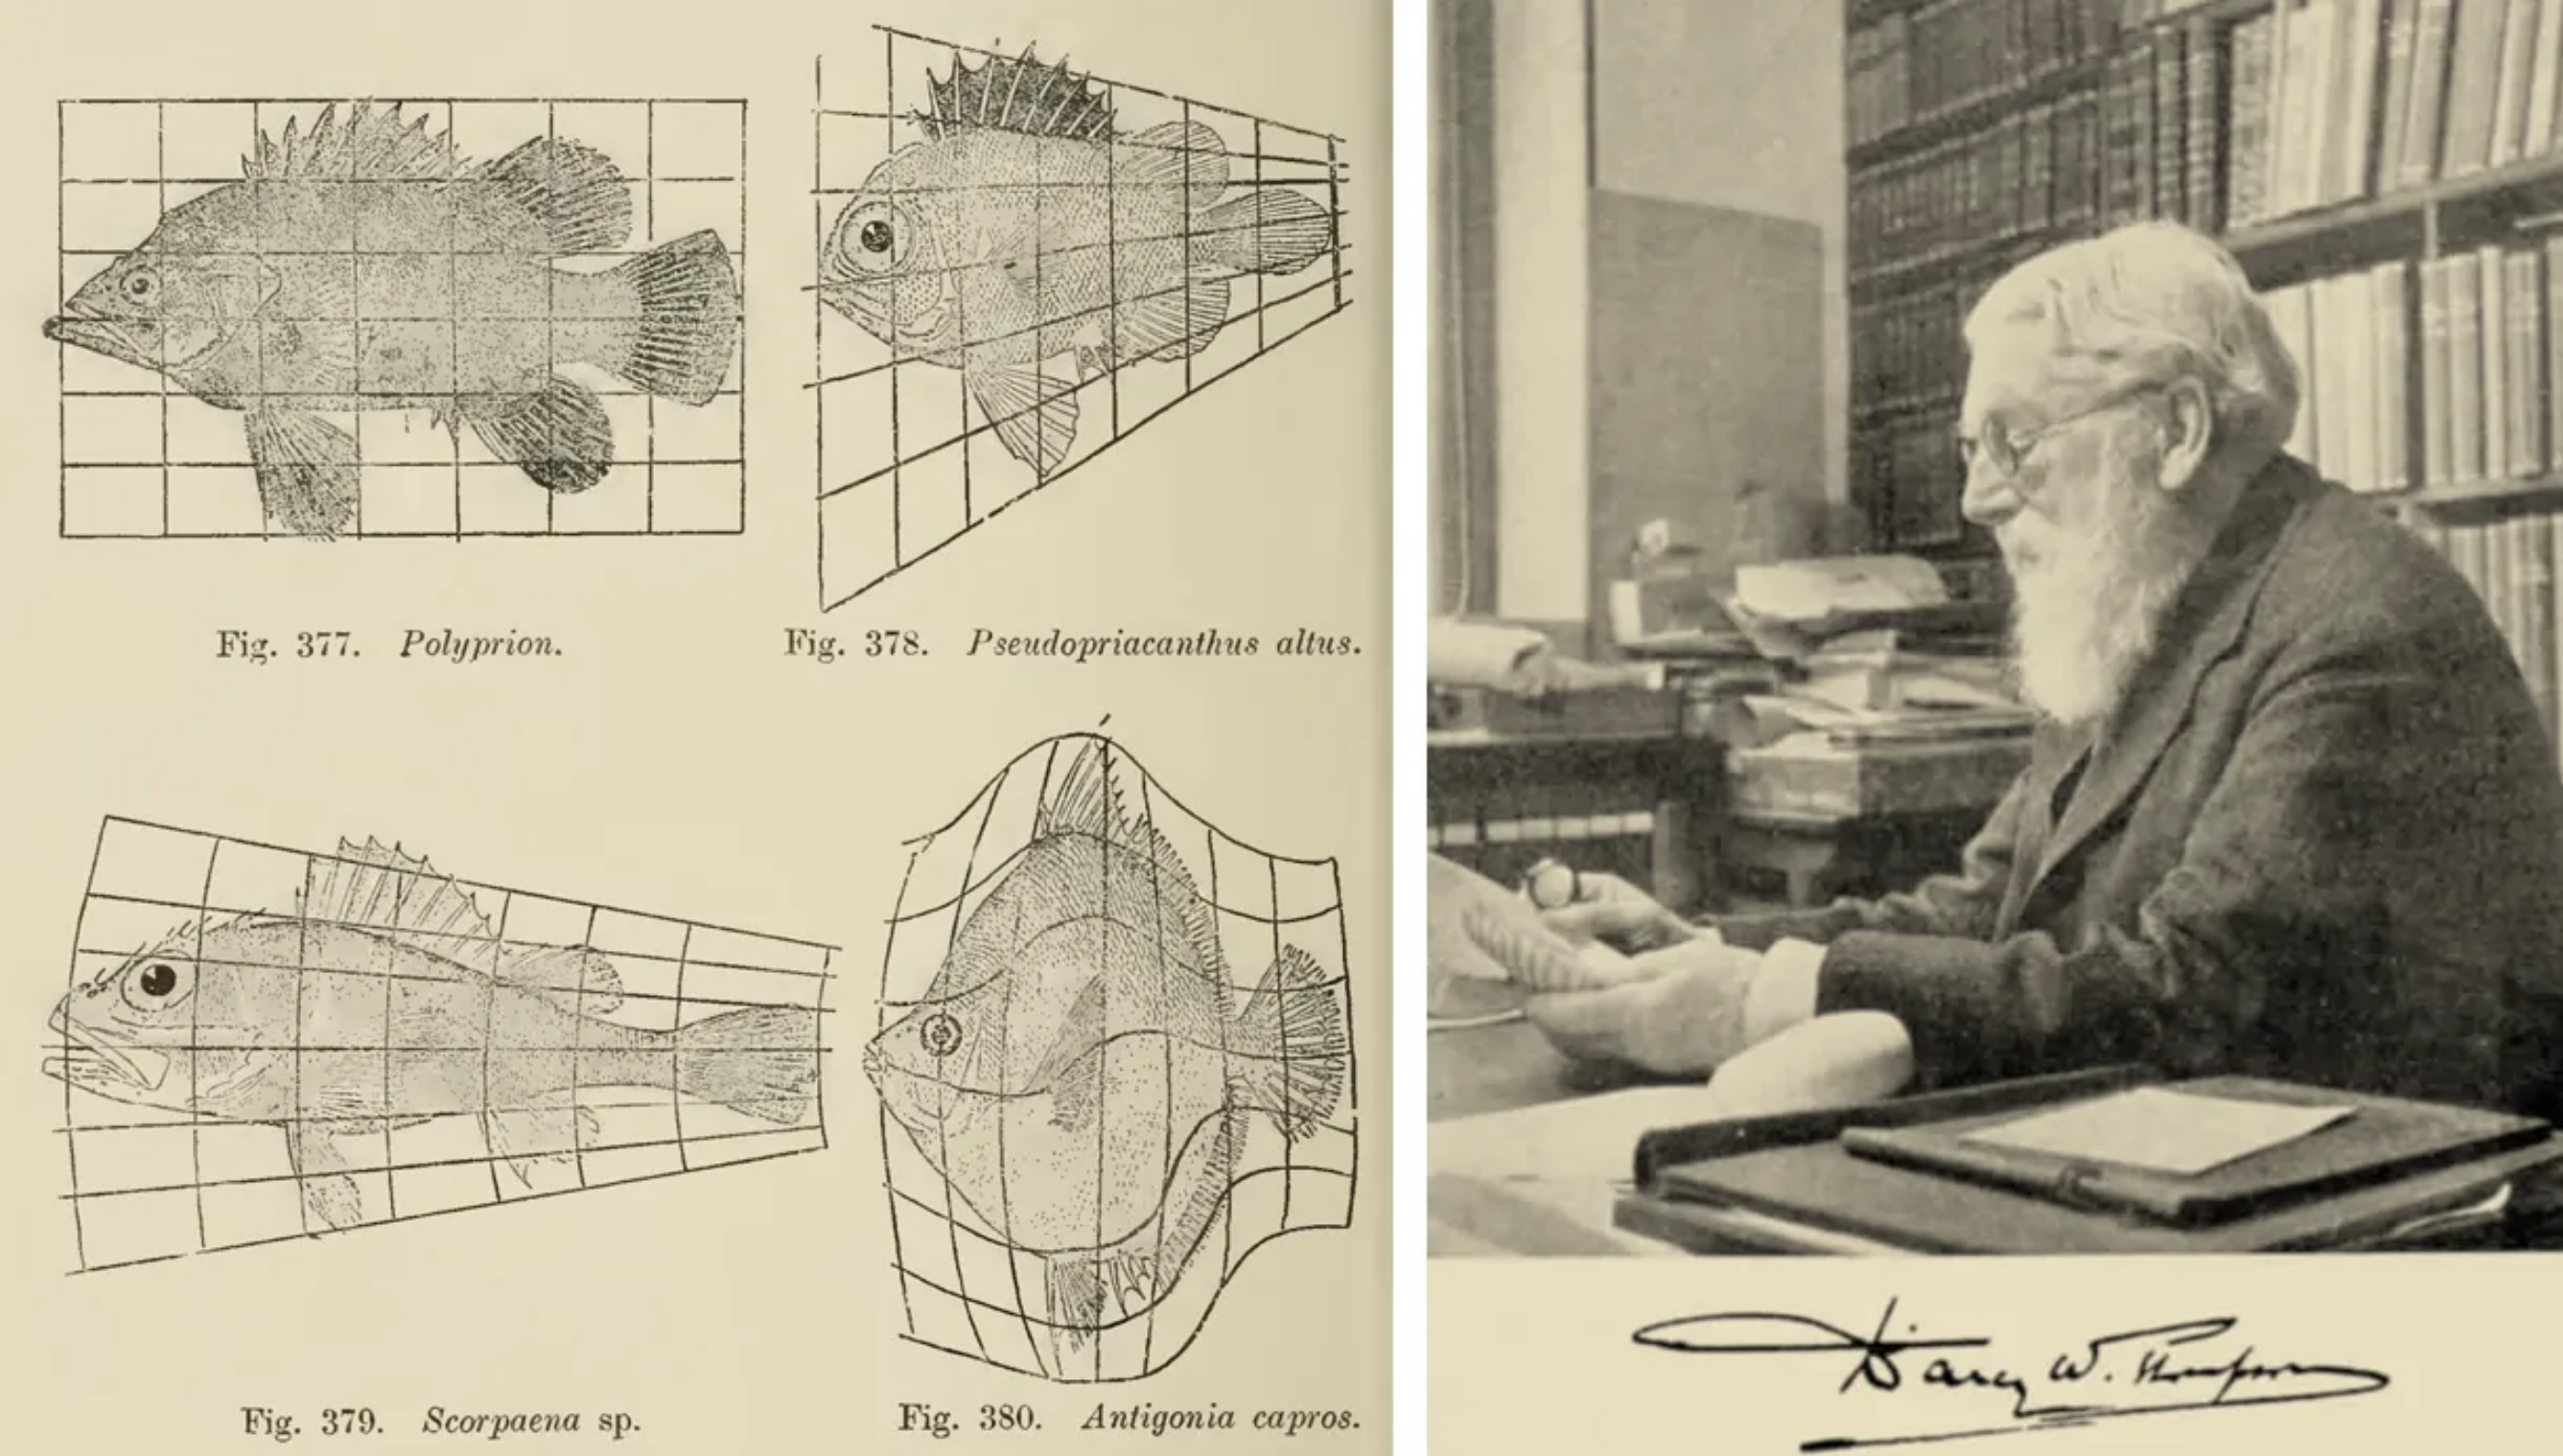
\includegraphics[width=0.6\textwidth]{chap2darcy.png}
	\caption{\label{fig_2_1b} \textbf{D'Arcy Thompson's fishes} and his theory of transformation. \cite{wolfram2017, thompson1979}}
\end{figure}

Thompson's work continues to inspire researchers even today. Right as I began my Ph.D., the centenary of the book's publication was being celebrated in the fields of developmental biology and biophysics \cite{heer2017, nat2017, natphys2017}. Even more so by the field of mechanobiology, an interdisciplinary field that studies the role of biophysical forces in cell and tissue functioning. 

\hypertarget{mechanobiology}{%
\section{Mechanobiology}\label{mechanobiology}}

The cells within epithelial tissue can be viewed as mathematical systems that integrate multiple input cues to result in an output behavior. These inputs can be mechanical or chemical, such as the stretching of lungs or the presence of morphogen gradients during embryonic development. The outputs can include cell deformation, migration, differentiation, or proliferation \cite{kumar2017}. Some outputs can even feedback into the system as an input, such as when cells remodel the matrix \cite{malandrino2018}. Mechanochemical switches at the membrane, cell-cell junctions, or cell-matrix adhesions mediate the sensing of the environment, triggering a biochemical cascade that leads to a cellular response \cite{roca-cusachs2017}. This interplay between biochemistry and mechanics is known as mechanotransduction.

During morphogenesis, mechanotransduction occurs at various scales, ranging from a single cell to complex multicellular tissue. To understand the role of different variables, experiments at different scales are necessary. It has been observed that individual cells can sense their environment and respond by altering their behavior through mechanical or biochemical processes. Whereas, multicellular systems can transmit forces and information at a longer length scale, allowing for emergent characteristics such as collective migrations, oscillations, rearrangements, and even turbulent flows \cite{heer2017, lecuit2011,trepat2018}.

An excellent demonstration of the interaction between tissues and their environment is provided by the phenomenon of durotaxis. Epithelial cells can detect changes in the stiffness of the extracellular matrix and migrate towards areas of higher rigidity. This migration towards stiffer regions has been observed both \textit{in vitro}, where cells in a monolayer collectively expand and relocate to stiffer areas, and \textit{in vivo}, such as during the migration of neural crest cells in \textit{Xenopus laevis} \cite{sunyer2016, shellard2021}. It is worth noting that the migration of neural crest cells themselves generates the durotactic gradient. In another example, during Drosophila oogenesis, the disorganized matrix is remodeled by cells to create a polarized matrix that aligns with the actin bundles in the follicular epithelium. This alignment is achieved through the coordinated rotation of cells and can guide the directed motion of cells along the polarized fibers \cite{haigo2011, cetera2014}.

The interplay between individual cells, their neighbors, and exogenous stimuli makes it difficult to decouple various biophysical aspects of the environment, such as forces, pressures, matrix stiffness, spatial confinement, porosity, or viscoelasticity. Direct force measurements in and out of tissues are also challenging. To address these challenges, researchers from various disciplines have attempted to recreate experimental systems with precise control over the biochemical and mechanical environments of cells \cite{xi2018}. This has been made possible through continuous technological advancements in fluorescent probes, imaging, microfabrication, and force measurements \cite{roca-cusachs2017}. In the following section, I will provide an overview of relevant techniques and experiments in the field of mechanobiology.

\hypertarget{synthetic-substrates}{%
\subsection{Synthetic substrates}\label{synthetic-substrates}}

The use of Polyacrylamide and soft PDMS gels has enabled researchers to investigate mechanical interactions at cell-substrate adhesion (see fig \ref{fig_2_2} A). Simply seeding cells on hydrogels of different stiffnesses reveals a significant impact on the actin cytoskeleton, cell shape, and lineage specification \cite{yeung2005,  engler2006}. These substrates, because of their known elastic response, are also utilized in techniques like traction force microscopy (TFM) to measure the forces exerted by cells and tissues on the substrate \cite{harris1980,  gomez-gonzalez2020} (see fig \ref{fig_2_2} D). TFM studies have shown that cells and tissues can exert greater forces on stiffer substrates as a result of the remodeling of the cytoskeleton \cite{elosegui-artola2016}. Higher matrix stiffness has also been found to induce the translocation of Yes-associated protein (YAP) from the cytoplasm to the nucleus, which is considered a sensor for mechanotransduction \cite{elosegui-artola2017}. However, increasing extracellular matrix (ECM) ligand density alone can induce YAP nuclear translocation without changing substrate stiffness \cite{stanton2019}.

\hypertarget{geometric-control}{%
\subsection{Geometric control}\label{geometric-control}}

The shape of cells or tissues on 2D substrates can be controlled using micropatterned adhesion proteins or microfabricated stencils. Protein patterning techniques are used to pattern adhesion promoting proteins and control cell attachment and spreading, while microfabricated stencils physically confine cells in a particular geometry (see fig \ref{fig_2_2} B C). When cells are confined, they respond by reorganizing their actin cytoskeleton and focal adhesion complexes to match the shape imposed on them \cite{vignaud2012}. Confined tissues undergo larger-scale rearrangements, leading to the formation of fascinating topological defects or oscillations \cite{tlili2018,  balasubramaniam2021,  guillamat2022}. Through these experiments, we can uncover the mechanisms of force transmission and regulation of collective cell migration and epithelial growth in two dimensions \cite{nelson2005,  vedula2012,  deforet2014}.

Embryonic stem cells subjected to 2D confinement have been shown to differentiate based on the shape and size of the confinement. For example, a circular monolayer of stem cells can reproduce the tissue patterning of a 3D gastruloid \cite{warmflash2014}, and confinement in a triangular shape can lead to high tension at the vertices and activate Wnt signaling, promoting differentiation to mesoderm \cite{muncie2020}. Moreover, advancements in photopatterning technologies allow for precise control of multiple proteins on the same substrate \cite{guyon2021, prahl2022}, enabling the establishment of complex co-culture systems that mimic \textit{in vivo} events.

Not just 2D shape, epithelial monolayers are also able to respond to curvature by regulating cell migration, orientation, cell/nucleus size, and shape \cite{marin-llaurado2022, schamberger2022} (see fig \ref{fig_2_2} C). For example, an epithelial monolayer on hemispheres of elastomers acts as a fluid with increasing curvature \cite{tang2022}. On a smaller scale, cells attached to corrugated hydrogels show variations in lamins, chromatin condensation, and cell proliferation rate in response to curvature \cite{luciano2021}. Bio-printing of three-dimensional tissue architectures can also create functional tissues \cite{brassard2021,  breau2022}.

\begin{figure}[h!]
	\centering
	\includegraphics[width=\textwidth]{chap2mechnobiology.png}
	\caption{\label{fig_2_2} \textbf{Mechanobiological strategies for studying morphogenesis} \textit{Adapted from \cite{vianello2019}}}
\end{figure}

\hypertarget{mechanical-control}{%
\subsection{Mechanical control}\label{mechanical-control}}

Living systems have mechanical control in addition to spatial control, as physical forces emerge from growth, deformation, and remodeling of the extracellular matrix (ECM) and fluid pressure in closed geometries. For example, the intestinal epithelia are stretched during peristaltic movements in the gut and lung alveoli deformations during breathing. Compression can also guide morphogenetic events that involve tissue bending and folding, such as the formation of the optic cup, gut villi, and cortical convolutions in the brain \cite{okuda2018, shyer2013, tallinen2016}.

To study tissue behavior under external perturbation, cells and tissues are probed at the molecular and subcellular scales using techniques such as atomic force microscopy, magnetic beads, optical tweezers, and micropipettes \cite{bao2003} (see fig \ref{fig_2_2} E). At a larger scale, various types of stretching devices, tissue rheometers, and force plates can be used \cite{xi2018}. These experiments reveal that cells exhibit complex viscoelastic behavior at different levels of deformation and different regions of the cytoskeleton \cite{mofrad2009}. The response of tissues to stretching can vary depending on the timescale of the stretch and the reorganization of
cells within the tissue \cite{guillot2013}. Rheological experiments also help to uncover the role of signaling pathways, such as YAP transcription factors, in mechanosensation \cite{wagh2021}.

The microfluidic system, also known as ``cells on a chip,'' has emerged as a valuable tool for investigating cell behavior under controlled biophysical conditions that mimic \textit{in vivo} conditions \cite{ingber2018}. This
system allows for the application of stretch or shear forces, as well as the creation of a controlled microenvironment that mimics the organ-level cues present in the body. For instance, the surface tension at the air-liquid interface in the lungs and the fluid flow through the vasculature, as well as the cyclic mechanical stretch of the tissue-tissue interface due to breathing, can be replicated using this approach \cite{huh2010}.

In the context of developmental biology, the use of microfluidic systems has allowed for the study of self-organization and embryo functions under controlled physical conditions. The co-culture of iPSC-derived motoneurons and brain microvascular endothelial cells in a microfluidic system has produced the \textit{in vivo}-like maturation of spinal cord neural tissue, representing a new avenue for exploring the complex interplay between physical and biological factors in development \cite{sances2018, samal2019}.

As mentioned earlier, the tissue-matrix interaction plays a critical role in sensing and rapidly transmitting forces \cite{tambe2011, sunyer2016, serra-picamal2012}. However, in early embryonic epithelia where little or no ECM is present, stresses generated by actomyosin contraction of the cells in one tissue are transmitted over long ranges via intercellular adhesions to other tissues. Thus, studying a simple free-standing epithelial monolayer is very appealing in terms of characterizing the mechanical response to stretch at different time scales.

Only two techniques are available for this: first, Harris and colleagues created a suspended monolayer by culturing a cell monolayer on a collagen matrix on two rods, and later removed the matrix using enzymatic digestion \cite{harris2012}. Second, epithelial domes, where MDCK cells pump ions to form fluid-filled blisters, have been used \cite{lever1979}. Recently, my colleagues, Ernest Latorre and Ariadna Marin-Llaurado, have enhanced control over the curvature, shape, and size of the domes \cite{latorre2018, marin-llaurado2022}, details on this system in the next chapter. These experiments showed that elasticity measurements of the monolayer were two orders of magnitude larger than those of individual cellular parts, and the monolayer could sustain more than 200\% strain before the rupture of cell-cell junctions. The cell cytoskeleton, particularly the actomyosin network and cadherin junctions, actively remodel during stretching, while the keratin network reinforces monolayer integrity at higher strains \cite{latorre2018, duque2023}. With sustained stretching, the tissue undergoes significant realignment and rearrangement via division \cite{wyatt2015}. Experiments on tissue devoid of the matrix also revealed epithelial actions such as superelasticity and buckling \cite{latorre2018, wyatt2020}.

\hypertarget{d-systems}{%
\subsection{3D systems}\label{d-systems}}

\textit{In vitro} experiments with 2D or 2.5D cell systems have improved our understanding of cell mechanics in morphogenesis by allowing us to measure deformations and forces and control environmental conditions that are inaccessible \textit{in vivo}. However, to gain a deeper understanding of cell mechanics, systems closer to the \textit{in vivo} environment must be probed.

Cell aggregates are a promising \textit{in vitro} system for probing cell mechanics, where synthetic matrix and mechanical measurement tools can be used. The response of cell clusters to the matrix, while similar to planar tissues, is more complex and includes sensitivity to matrix stiffness, confinement, and ECM concentration, as well as the ability to undergo 3D shape transformations (see fig \ref{fig_2_2} E). Our lab has demonstrated that cell aggregates perform durotaxis and exhibit wetting behavior dependent on stiffness \cite{perez-gonzalez2019, pallares2022}. Additionally, cell aggregates in suspension behave like viscous droplets and can be used to measure rheological properties, such as when squeezed between plates or probed with AFM or a micropipette \cite{xi2018}. The viscoelastic properties of cell aggregates can even be measured by coalescing two aggregates
\cite{oriola2022}.

In recent years, the use of hydrogel systems for the culturing cell aggregates has gained significant attention. Hydrogels, such as polyethylene glycol (PEG), polyacrylamide, collagen, or Matrigel, serve as a supportive environment for cell growth. Naturally extracted hydrogels like Matrigel provide a similar architecture to the native ECM. When embedded into a hydrogel, polarized epithelia tend to form a spherical structure with a hollow lumen, which can be induced to form branching morphogenesis by hepatocyte growth factor \cite{bryant2008}. 

Cell-driven self-assembly in organoids leads to tissue formation that mimics organ features, but achieving reproducibility in shape and composition is often challenging \cite{nelson2008, hofer2021}. Synthetic hydrogels with control over ligand presentation, crosslinking, and degradability have proven useful for epithelial organoids, allowing for control over cell fate \cite{gjorevski2016, gjorevski2022}.

3D gel-based culture systems with spatiotemporal control over the mechanical properties corresponding to \textit{in vivo}-like functional structures have also been developed \cite{torras2018}. Interestingly, recent publications show tissue transformation from planar to complex organ-resembling tissue without fine environmental control. For example, intestinal epithelium mechanically compartmentalizes itself, and 2D stem cells transform into a 3D neural tube \cite{perez-gonzalez2021, karzbrun2021}.

In developing embryos, both embryonic and extraembryonic fluids generate frictional and tensional stresses when flowing, or hydrostatic pressures when confined within spaces \cite{vianello2019, chan2020}. The challenge of measuring these forces has led to the use of various techniques, including micropipette aspiration. Micropipette experiments, where a needle is inserted into the embryo to control pressure, have revealed that the internal hydrostatic pressure determines the embryonic size and dictates cell fate allocation \cite{chan2019} (see fig \ref{fig_2_2} E). As a fluid-filled structure, the hydrostatic pressure inside the embryo corresponds to tension in its surfaces, and changes in luminal volumes are sensed by cells through increased cortical tension, inducing changes in cell shape and cytoskeleton organization \cite{chan2019, choudhury2022}. Micropipette aspiration has also been effective in measuring the surface tension of individual cells or whole blastomeres \cite{dumortier2019}, thus providing insight into the role of the actin cortex in regulating preimplantation embryonic contractility \cite{ozguc2022, firmin2022}.

The measurement of forces within embryos has also been approached through the insertion of deformable probes, such as hydrogels, oil, or magnetic droplets \cite{dolega2017, campas2014, serwane2017}. The shape changes of these probes allow for measurement of local forces and osmotic pressures \cite{mongera2023}.

In addition to embryos, explant systems have been utilized to study organogenesis in the brain, gut, and lungs. Lung explant research has been particularly useful in understanding different aspects of shape formation, which occurs under the influence of pressure and growth factors. The explant system allows for direct control over the chemical and mechanical environment at specific stages of development. Work with mouse airway epithelium has shown that pressure and matrix stiffness impact the number of lung branches \cite{palmer2021, varner2015, nelson2017}.

Other tools such as optical tweezers, laser ablation, and optogenetic excitations have been used at different levels to probe the mechanics of development \cite{lecuit2011, gomez-gonzalez2020}. However, independent control over multiple factors remains difficult and force measurement remains indirect.

In conclusion, epithelial tissues are highly sensitive to various biophysical forces and constantly undergo remodeling at different scales and timeframes. There are multiple techniques available to manipulate and study these tissues, from single cells to embryos, with controlled forces and deformation. Due to its dynamic behavior, epithelial tissue can be considered an active material. The focus of this thesis is to develop a system that can control and measure physical forces to understand epithelial behavior as an active material. In the following chapter, we will delve into the molecular machinery responsible for driving these active tissues.